\documentclass[UTF8,12pt]{article}

\usepackage[utf8]{inputenc}
\usepackage{ctex}
\usepackage{amsmath,amsfonts,amssymb}
\usepackage{graphicx,epsfig,subfig}
\usepackage{makeidx,hyperref}
\usepackage{geometry}
\usepackage{listings}
\usepackage[linesnumbered,boxed]{algorithm2e}
\usepackage{xcolor}

\geometry{scale=0.8}

%\setlength{\lineskip}{\baselineskip}
\setlength{\parskip}{0.5\baselineskip}

\title{Anderson局部化实验报告3}
\author{flag}
\date{\today}

\begin{document}
    
\maketitle

\section{文献大意}

文章搞了一个“有效势”,可以用来估计局部化的特征函数的边界。并且根据这个给出了weyl公式来估计特征值的具体值。

\subsection{解释指数收敛的现象}

特征值问题
$$ - \Delta \psi(x) + V(x) \psi(x) = E \psi(x) $$
其中,$\psi(x)$是归一化到最大值为1的特征函数。

源项问题
$$ - \Delta u(x) + V(x) u(x) = 1 $$
定义$W = 1/u$就是“有效势”。

引入辅助函数$\phi$满足$\psi = u \phi$,特征值问题就化为
$$ - \Delta (u \phi) + V u \phi = E u \phi $$
展开,把$V u = 1 + \Delta u$代入得到
$$ - \frac{1}{u^2} div(u^2 \nabla \phi) + W \phi = E \phi $$
这相当于一个势函数为W的新型椭圆方程。

如果是不用考虑边界上积分的情况(Dirichlet边界,Neumann边界还有周期边界)。两边乘以$u^2 \phi$之后积分得到
$$ \|u \cdot \nabla (\frac{\psi}{u})\|^2 + (W \psi, \psi) = E \|\psi\|^2 $$
这说明,如果归一化到$\|\psi\|^2 = 1$,那特征函数对应的特征值就可以满足$E < (W \psi, \psi)$。

这个方程还表明,在$E < W$的地方,$W$和$E$之间的差可以定义一个Agmon距离$\rho_E(x_1, x_2)$,它可以控制$\psi$在这些区域处的下降。(不知道这个结论数学上的解释是什么样的)

距离的定义为
$$ \rho_E(x_1, x_2) = \min_\gamma \int_\gamma \sqrt{(W(x)-E)_+} \; ds $$
其中$\gamma$是$x_1$到$x_2$的所有路径。

结论是
$$ |\psi(x)| \leqslant e^{\rho_E(x_0, x)} $$
这个结论在数学上怎么推的我也不知道。

\begin{figure}[htbp]
\centering
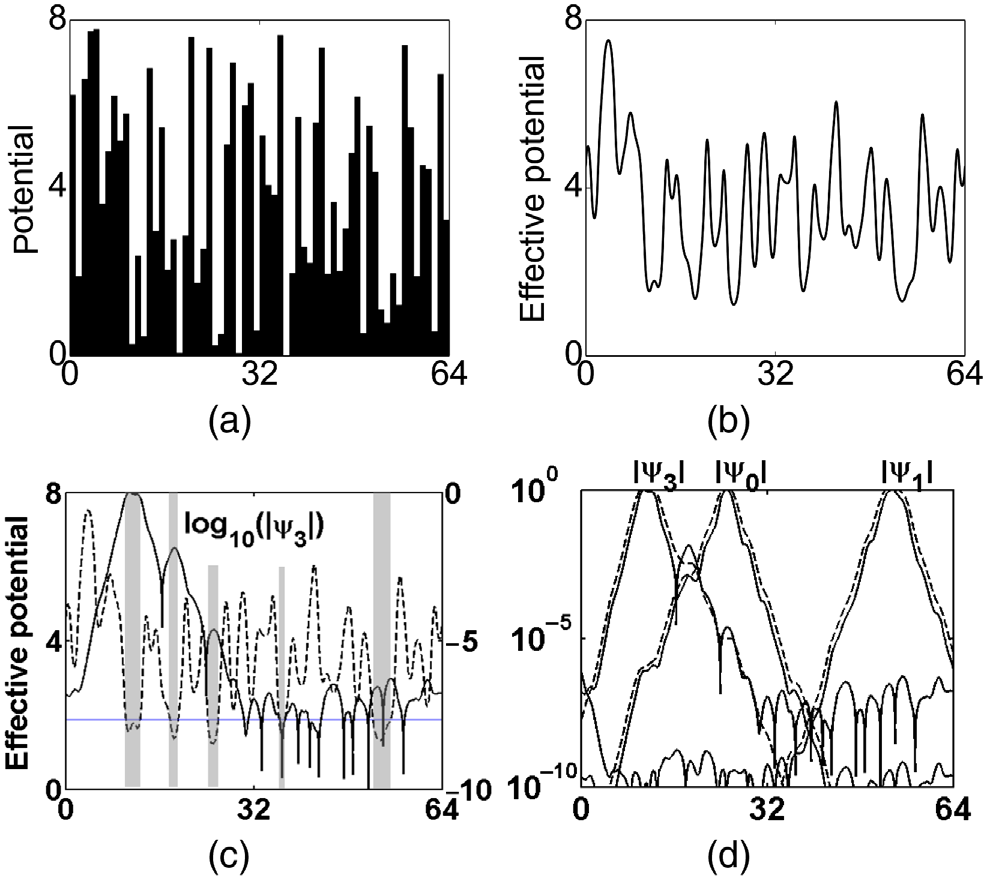
\includegraphics[width=0.7\linewidth]{article1}
\caption{文章里的figure1}
\label{article1}
\end{figure}

通过数值模拟来验证这个结论。图\ref{article1}是文章里的图。其中(a)是势函数V的图像,(b)是$W = 1/u$的图像,(c)中灰色部分是$W<E$的部分,这部分$\psi$没有衰减,在白色的部分,$\psi$有指数衰减。(d)中实线是三个特征函数的图像,虚线是$e^{\rho_E}$的图像。可以看出在$\psi$比较大的时候,这个估计还是特别准的。(边界条件为周期边界)

后面模拟了二维的情况,二维的情况就是valleyline来划分位置了,$1/u$仍然可以控制特征函数的指数下降。图\ref{article1}是文章里的图。其中(a)是势函数V的图像,(b)是$W = 1/u$的图像,和valleyline。(c)是$\log_{10} (\psi_0)$的图像。(d)是$\log_{10} (|\nabla \psi|)$的图像。(边界条件好像也是周期边界。)

(PS:这里说画出valleyline是用watershed算法画出来的,那是啥算法?)

(PPS:这个文章里实验的都是K比较小的情况,没提到K很大时候的情况,不知道K大了会咋样。)

\begin{figure}[htbp]
\centering
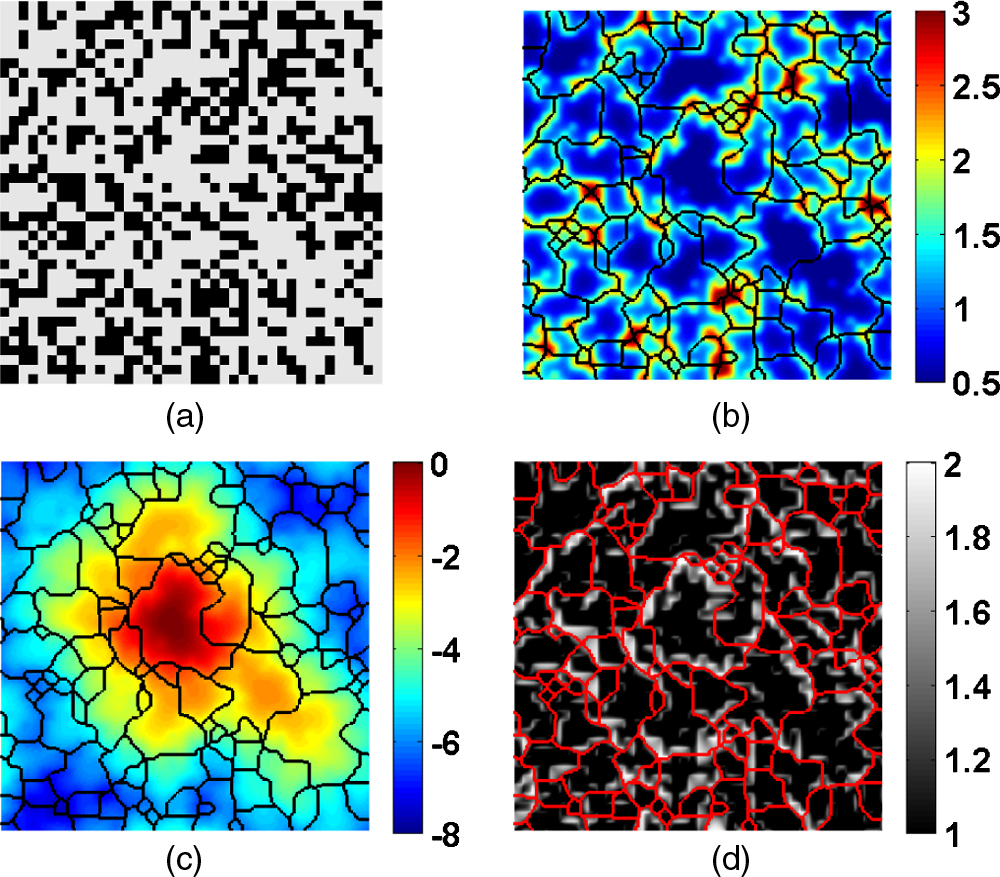
\includegraphics[width=0.7\linewidth]{article2}
\caption{文章里的figure2}
\label{article2}
\end{figure}

最后的结论大概是,valleyline相当于阻碍量子效应传播的障碍,量子隧穿效应使特征函数在穿过valleyline的时候指数衰减。用W控制特征函数的方法和之前PNAS里的文章差不多。当特征值大于W的最大值的时候,量子化就失效了。

\subsection{修正的weyl定理}

“有趣”的事情是,W可以看成是势函数V的光滑化。因为有这个式子
$$ V - W = \frac{\Delta u}{u} $$

Weyl定律告诉我们,某个特征值对应的“态密度”(我猜可能是小于E的特征值个数)$N(E)$可以用这个公式近似
$$ N(E) \approx (2 \pi)^{-n} \int_{k^2 + V(x) \leq E} \ dx dk $$
这里的$n$是空间维数。它在E很大的时候渐进地准确。

一维的Weyl定律就可以写成
$$ N_V(E) = \frac{1}{\pi} \int_{E > V(x)} (E - V(x))^{1/2}  \ dx $$
文章里说这个东西在E比较小的时候不准,就把这里面的V换成了W,得到$N_W(E)$,经过模拟证明,这样换完之后,预测特征值准确多了。

图\ref{article3}是文章里的图。其中左边是势函数V的图像,右边是$N(E),N_V(E),N_W(E)$的图像。可以明显地看到$N_W$更加准确一些。

\begin{figure}[htbp]
\centering
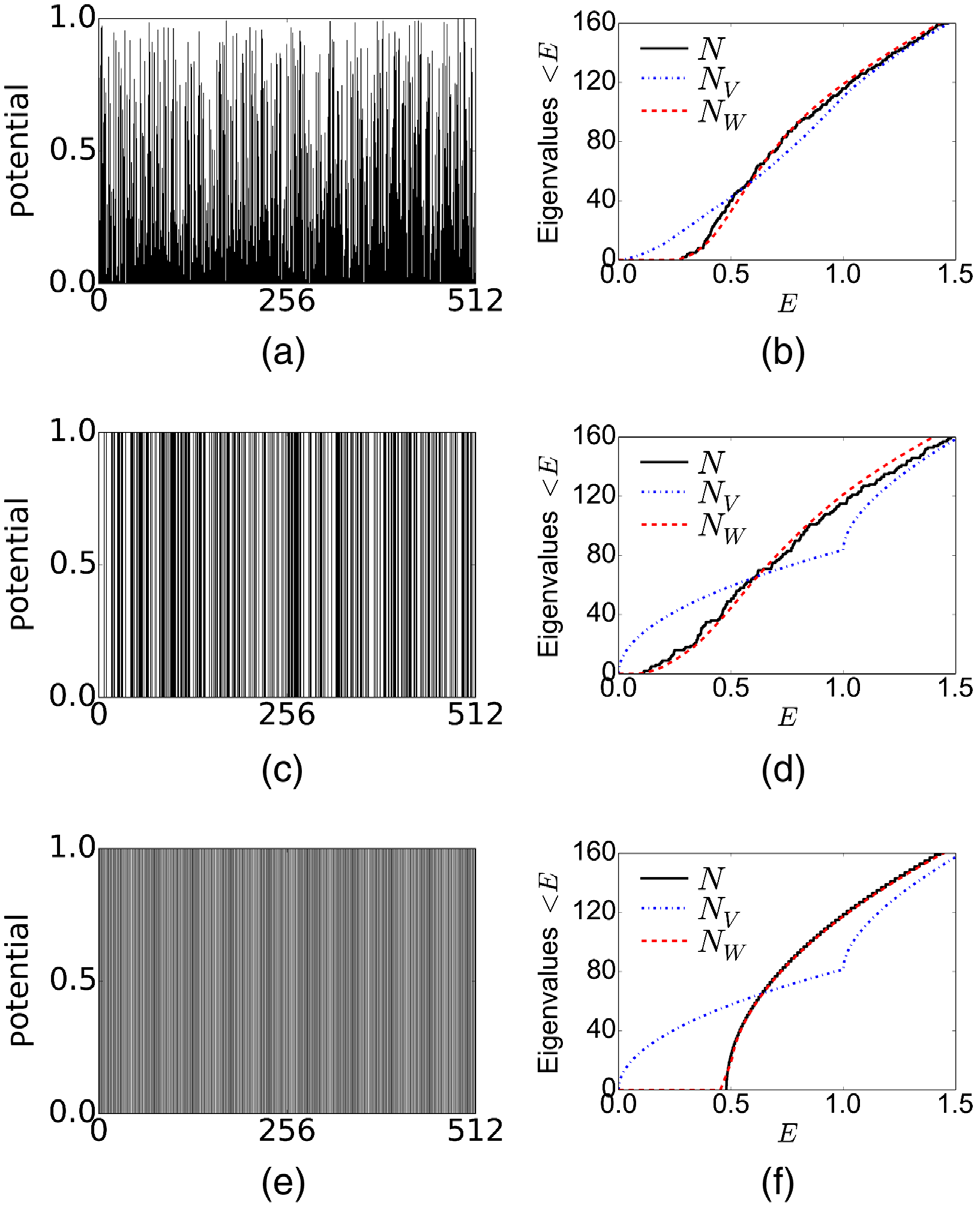
\includegraphics[width=0.7\linewidth]{article3}
\caption{文章里的figure3}
\label{article3}
\end{figure}

这个weyl定理文章里没有二维的情况,可能是由于之前我们模拟的结果,二维情况下不同边界条件对特征值影响很大。

\newpage

\section{在其他边界条件下的推广}

文章中说结论适用于Dirichelt边界,Neumann边界,周期边界。更细致的推导我也不知道,但是就文章中写出来的结果来看,和边界条件有关的地方只有一个,就是计算这个的时候。
$$ - \int_\Omega div(u^2 \nabla \phi) \ \phi \ dx = \int_\Omega |u \nabla \phi|^2 \ dx - \int_{\partial \Omega} u^2 (\nabla \phi \cdot \mathbf{n}) \phi \ dx $$
边界上的项可以化为
$$ u^2 (\nabla \phi \cdot \mathbf{n}) \phi = \phi \ (\frac{\partial \psi}{\partial \mathbf{n}} u - \frac{\partial u}{\partial \mathbf{n}} \psi) $$
如果特征值问题是Robin边界,就是
$$ \frac{\partial \psi}{\partial \mathbf{n}} + h \psi = 0 $$
这个时候想要消掉边界,landscape函数$u$也要满足一样的边界条件
$$ \frac{\partial u}{\partial \mathbf{n}} + h u = 0 $$
这个和之前我们对landscape提的边界条件不一样,这里就难以推广了。

\end{document}